\subsection{Der Eventbus}
\todo{Deadline: 25.06.}

Der \emph{Eventbus} stellt für Softwarekomponenten die Möglichkeit bereit, Ereignisse untereinander auszutauschen. Für jedes Ereignis stellt er eine $m$:$n$-Beziehung zwischen den Komponenten, welche das Ereignis emittieren und denen, die es empfangen her. Der \emph{Eventbus} wurde in Zusammenarbeit mit \citeauthor{persitzky_fehlerinjektion_2023} entwickelt. Wir haben uns dazu entschieden, das Entwurfsmuster \emph{Mediator} auf den \emph{Eventbus} anzuwenden, um zu verhindern, dass die voneinander Abhängigen Komponenten direkt miteinander kommunizieren müssen. Das senkt die Kopplung erheblich. Weiterhin kapselt der \emph{Mediator} das kommunikationsspezifische Verhalten, was es an einer zentralen Stelle verfügbar macht und den einzelnen Komponenten die Verantwortung abnimmt, Kommunikationsdetails zu kennen.\\
\\
Um eine zu große Komplexität des \emph{Eventbus} selbst und eine monolithische Struktur zu verhindern, wird als Kommunikationsmechanismus das Entwurfsmuster \emph{Observer} verwendet. Abhängigkeiten zwischen den Komponenten lassen sich so flexibler ändern. Weiterhin ermöglicht dieses Entwurfsmuster, Komponenten auf verschiedenen Abstraktionsniveaus zu verbinden. Wir haben den Nachteil des \emph{Observers} umgangen, dass er stets alle Empfänger benachrichtigt. Dazu wird jeder registrierte Empfänger mit einem Ereignistyp verknüpft. Der Empfänger wird so nur benachrichtigt, wenn ein Ereignis des verknüpften Typs eingangen ist.\\
\\
Um die Kopplung weiter zu verringern, werden beim \emph{EventBus} nicht die Empfänger selbst registriert, sondern nur \emph{Callbacks}\footnote{Funktionen, welche als Argument übergeben werden, um zu einem späteren Zeitpunkt vom Empfänger des Arguments aufgerufen werden zu können}, bei welchen es sich jeweils um Methoden der Empfänger handelt. Dies schränkt die Funktionalität nicht ein, da der Empfännger das Ereginis nachwievor erhält. Der \emph{Eventbus} muss nun jedoch nur noch Pythons \code{Callable}-Schnittstelle verwenden und benötigt keine Kenntnis mehr über die Kommunizierenden Komponenten. Die Registrierung und die Deregistrierung von Empfängern ist in den Abbildungen \ref{fig:eventbus-register-seq} und \ref{fig:eventbus-unregister-seq} dargestellt. Für die Registrierung wird das \emph{Callback} und der Ereignistyp (\code{event\_type}) übergeben. Der \emph{Eventbus} gibt daraufhin ein \emph{Handle} zurück, mit welchem das registrierte \emph{Callback} identifiziert werden kann. Um ein \emph{Callback} zu deregistrieren, lediglich das \emph{Handle} and den \emph{Eventbus} übergeben werden.

\begin{figure}[!hb]
	\centering
	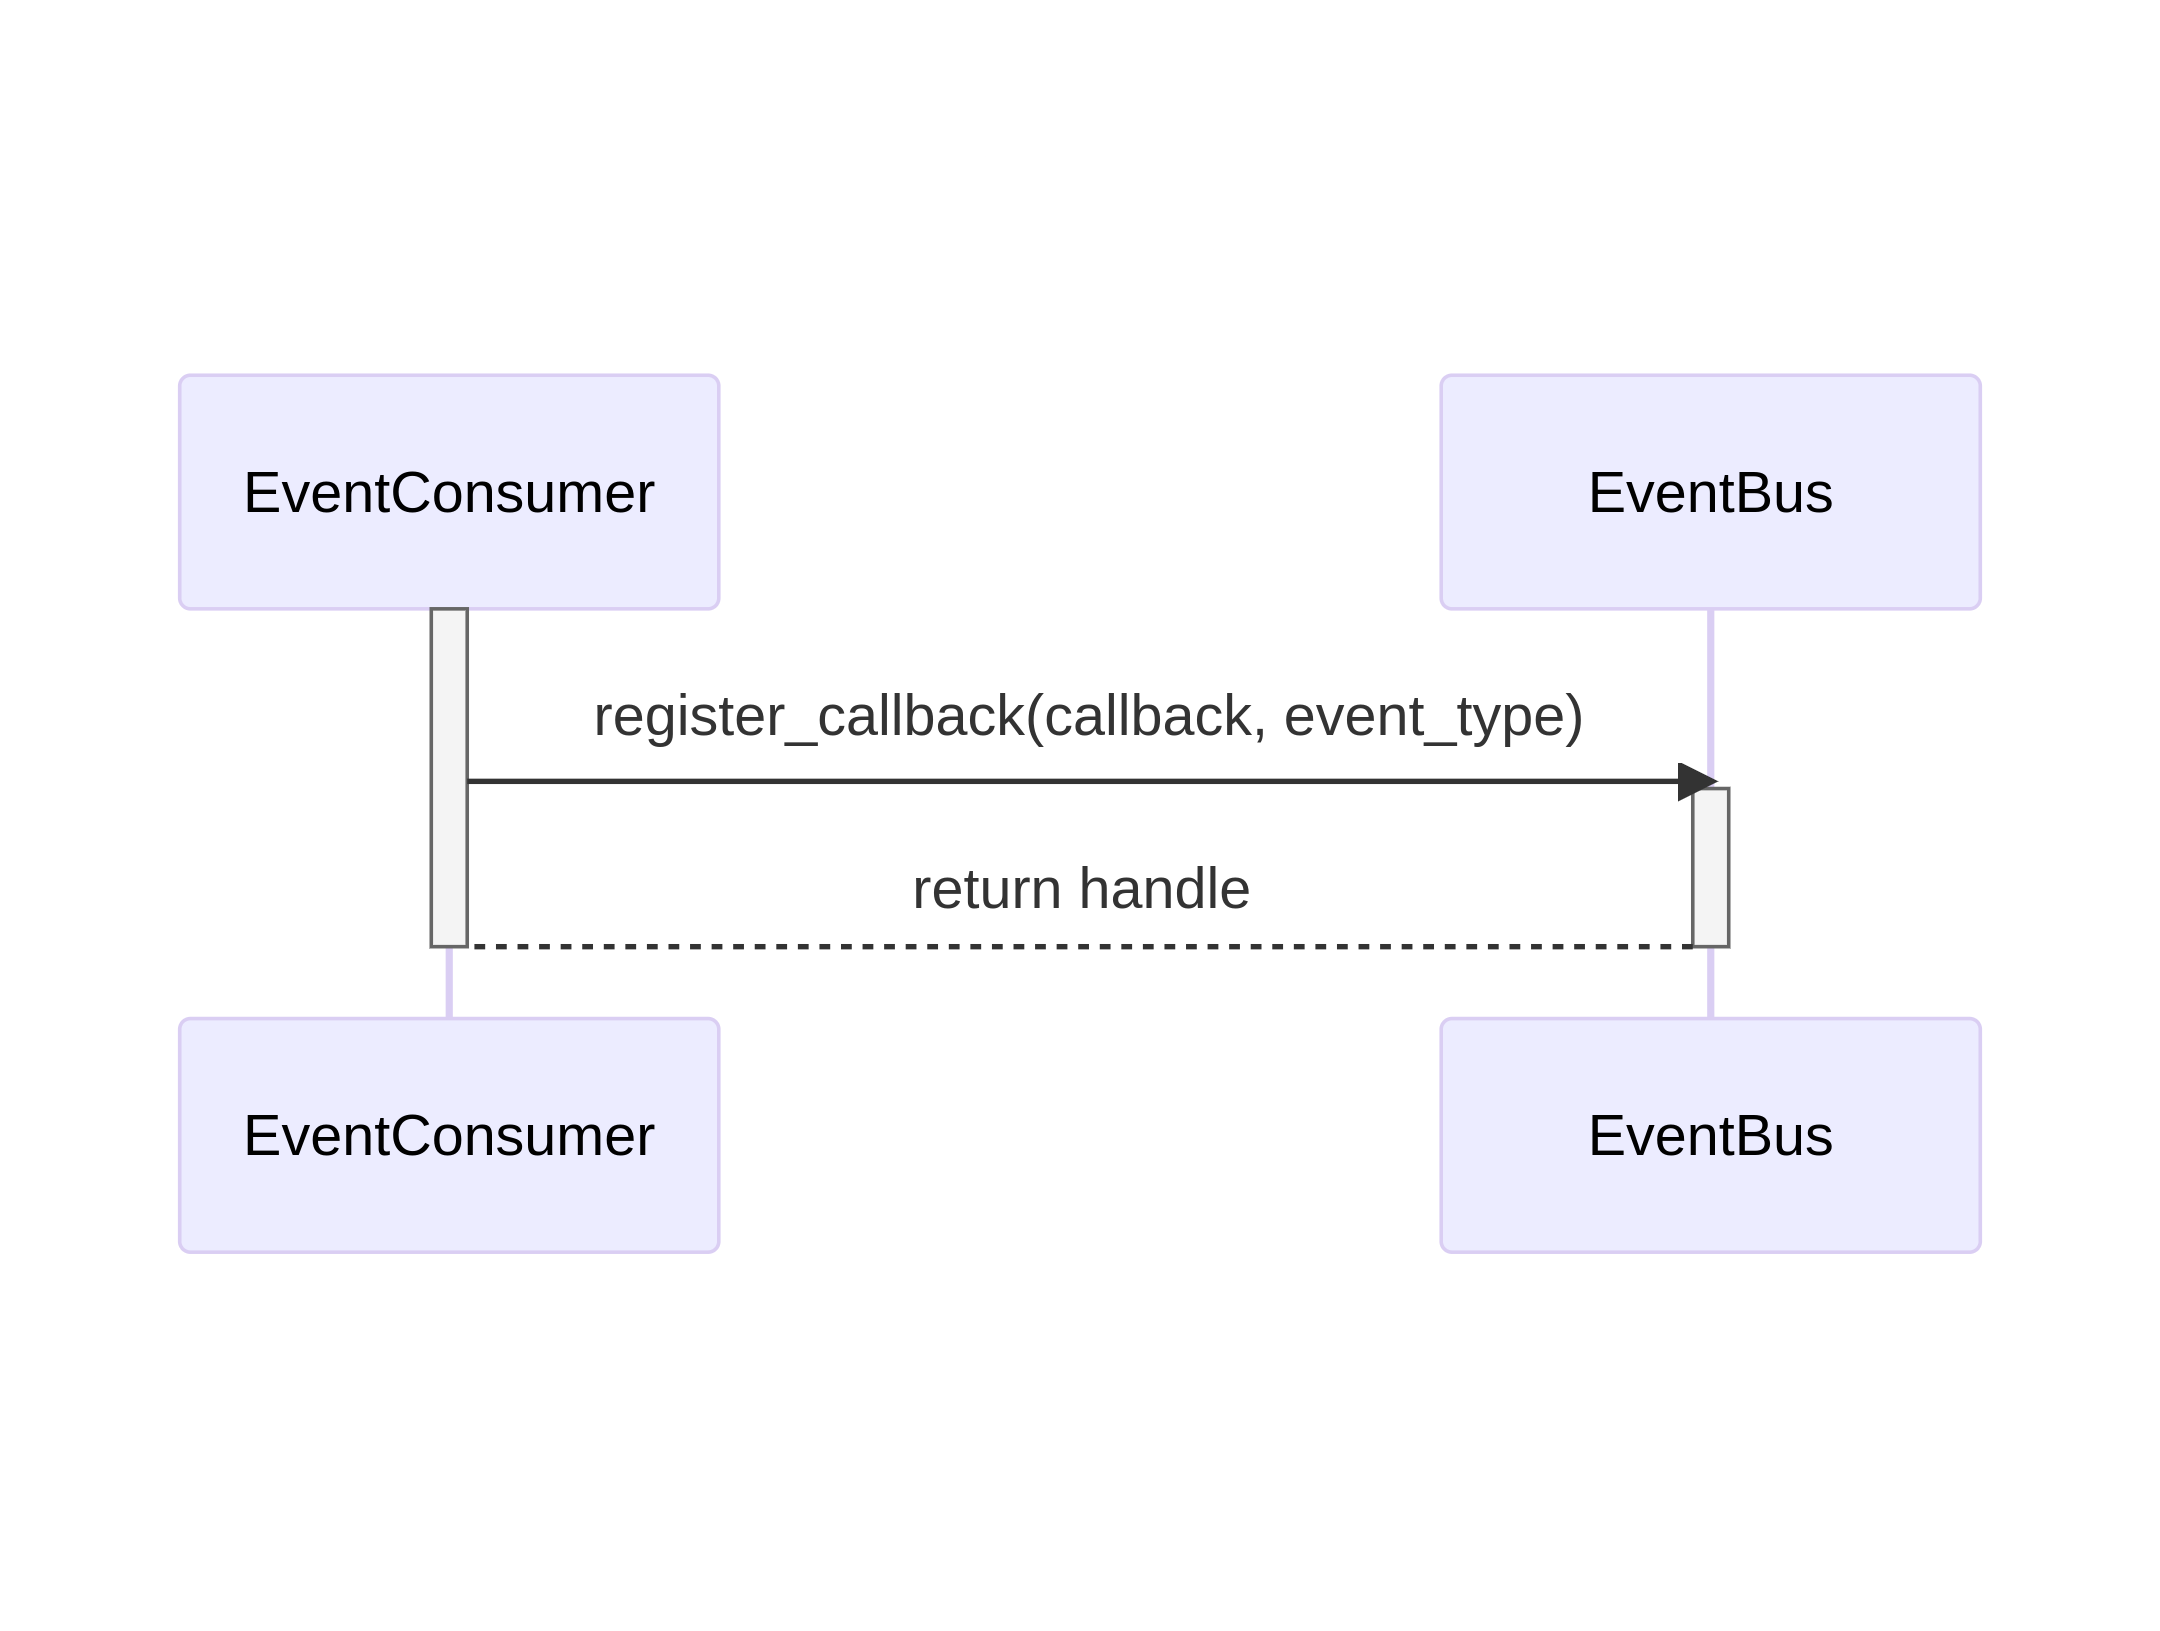
\includegraphics[width=0.75\linewidth]{images/diagrams/eventbus-register-seq.png}
	\caption{Sequenzdiagramm Registrierung Eventbus}
	\label{fig:eventbus-register-seq}
\end{figure}

\begin{figure}[!hb]
	\centering
	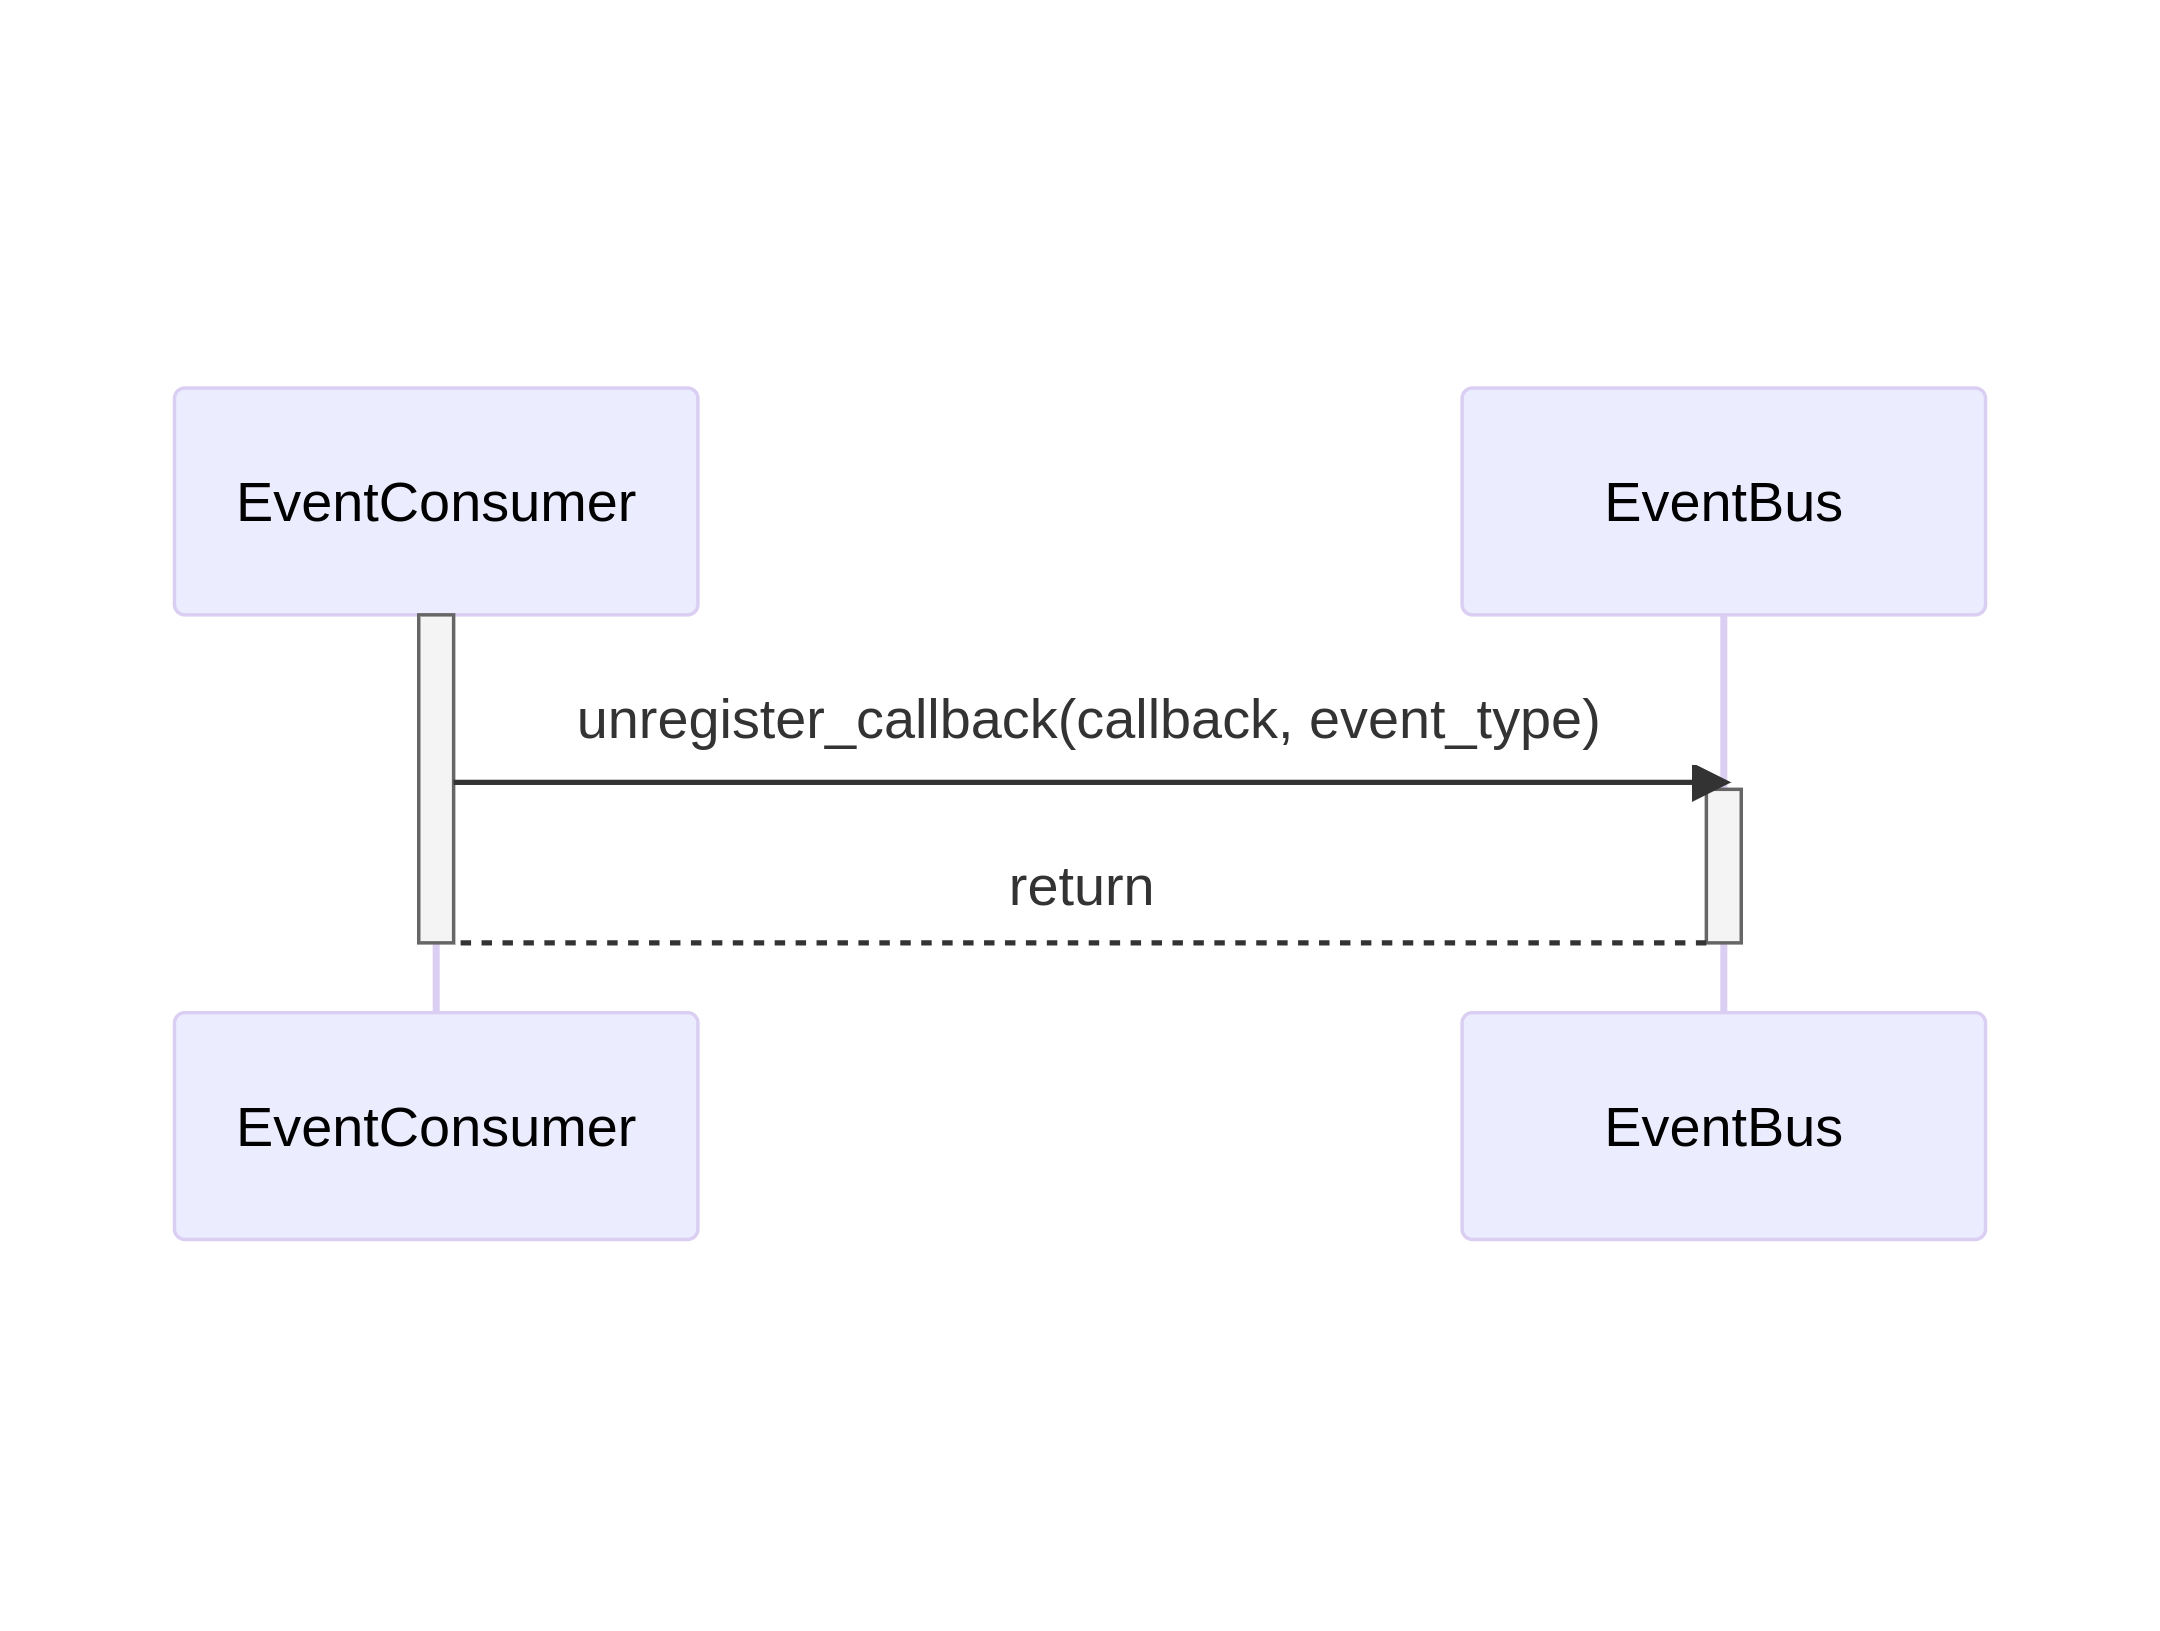
\includegraphics[width=0.75\linewidth]{images/diagrams/eventbus-unregister-seq.png}
	\caption{Sequenzdiagramm Deregistrierung Eventbus}
	\label{fig:eventbus-unregister-seq}
\end{figure}

Die Implementierung des \emph{Eventbus} erfolgte vergleichsweise spät im Projektverlauf. Die Codebasis war bereits entsprechend groß, was uns vor die Herausforderung stellte, wie der \emph{Eventbus} am besten zu integrieren sei. Auch spielte die Zeitplanung dabei eine Rolle.\\
\\
Da der \emph{Logger}\cite{reisener_entwurf_2023} bereits die Aufgabe übernahm, Ereignisse zu sammeln, lag der Gedanke nahe, ihn entsprechend zu erweitern. Diese Möglichkeit ist im Folgenden unter ''Variante 1'' beschrieben.\\
\\
Da diese Variante gewisse Nachteile mit sich bringt, wird unter ''Variante 2'' eine architektonisch sauberere Lösung vorgestellt. Für diese zweite Lösung haben wir uns aus unten genannten Gründen letztendlich entschieden.

\subsubsection*{Variante 1}

Bei dieser Variante wird das System des \emph{Loggers} erweitert, um die Aufgaben des \emph{Eventbus} zu übernehmen. Wie Abbildung \ref{fig:eventbus-v1-class} zeigt, erstellt der \emph{Logger} für jedes Ereignis ein \code{LogEntry}-Objekt, welches in die Datenbank geschrieben wird. Das \code{LogEntry}-Objekt erbt daher von \code{BaseModel} und besitzt eine \code{save}-Methode, welche bei Erzeugung des Objektes stets ausgeführt wird.

\begin{figure}[!hb]
	\centering
	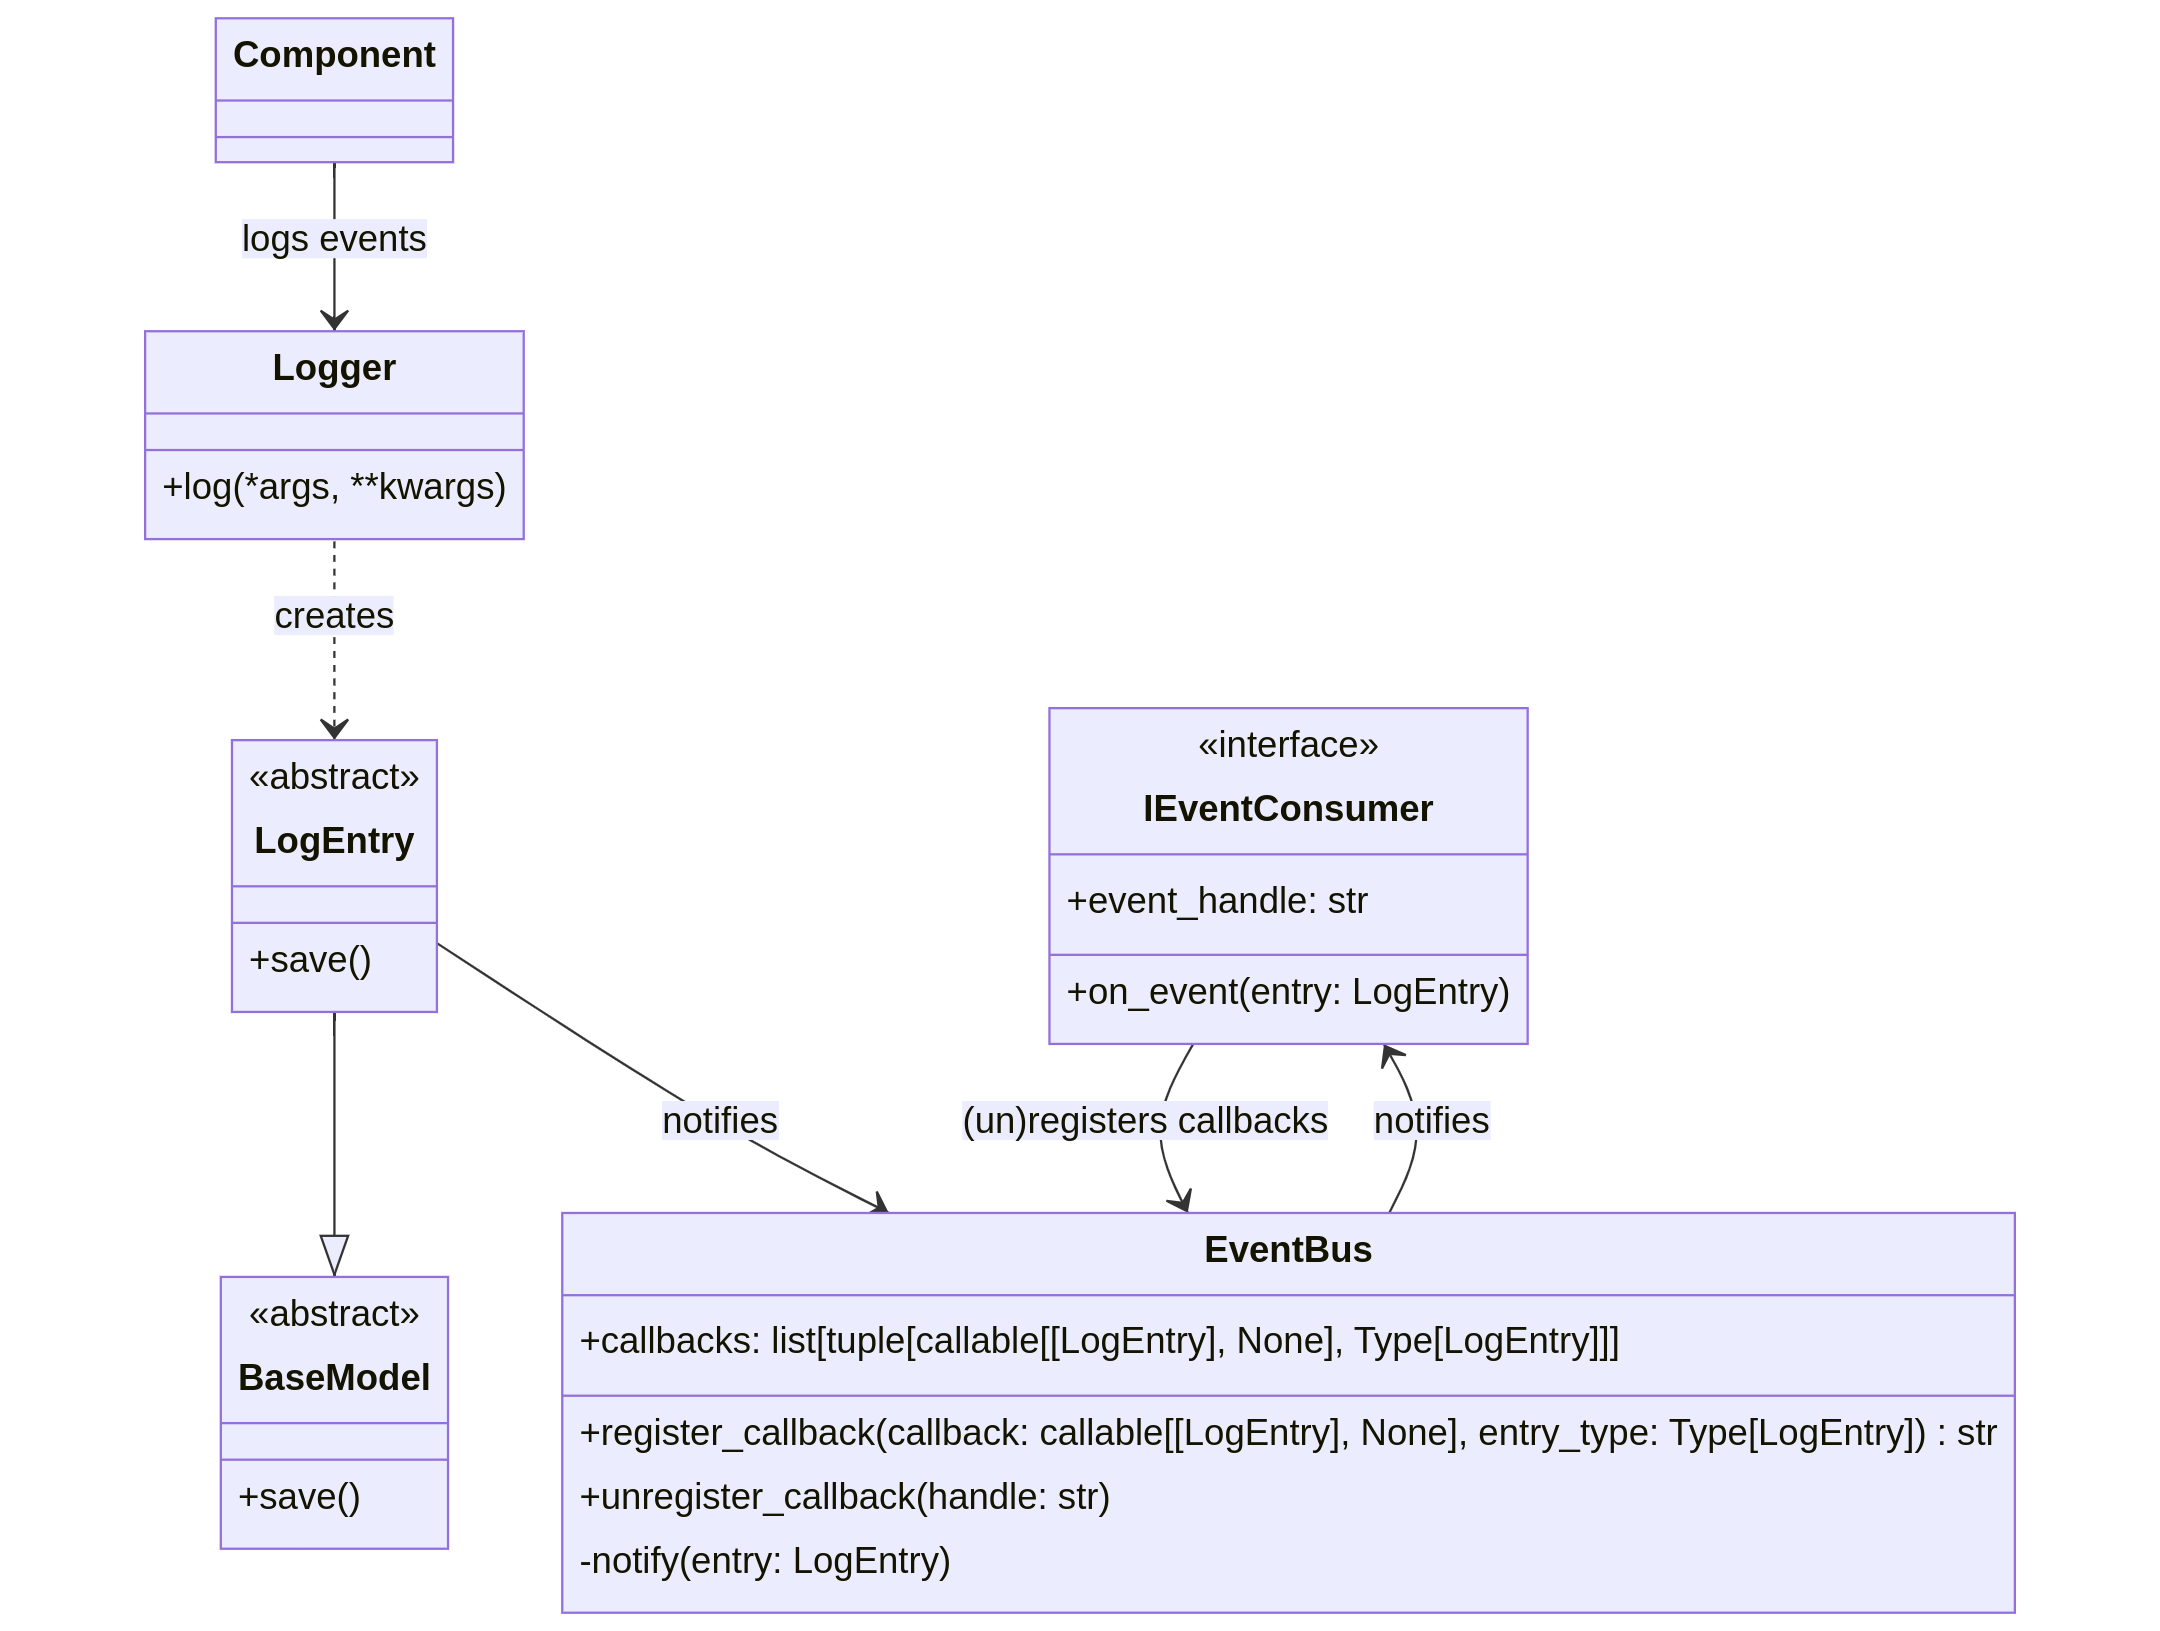
\includegraphics[width=0.75\linewidth]{images/diagrams/eventbus-v1-class.png}
	\caption{Klassendiagramm Variante 1 Eventbus}
	\label{fig:eventbus-v1-class}
\end{figure}

\begin{figure}[!hb]
	\centering
	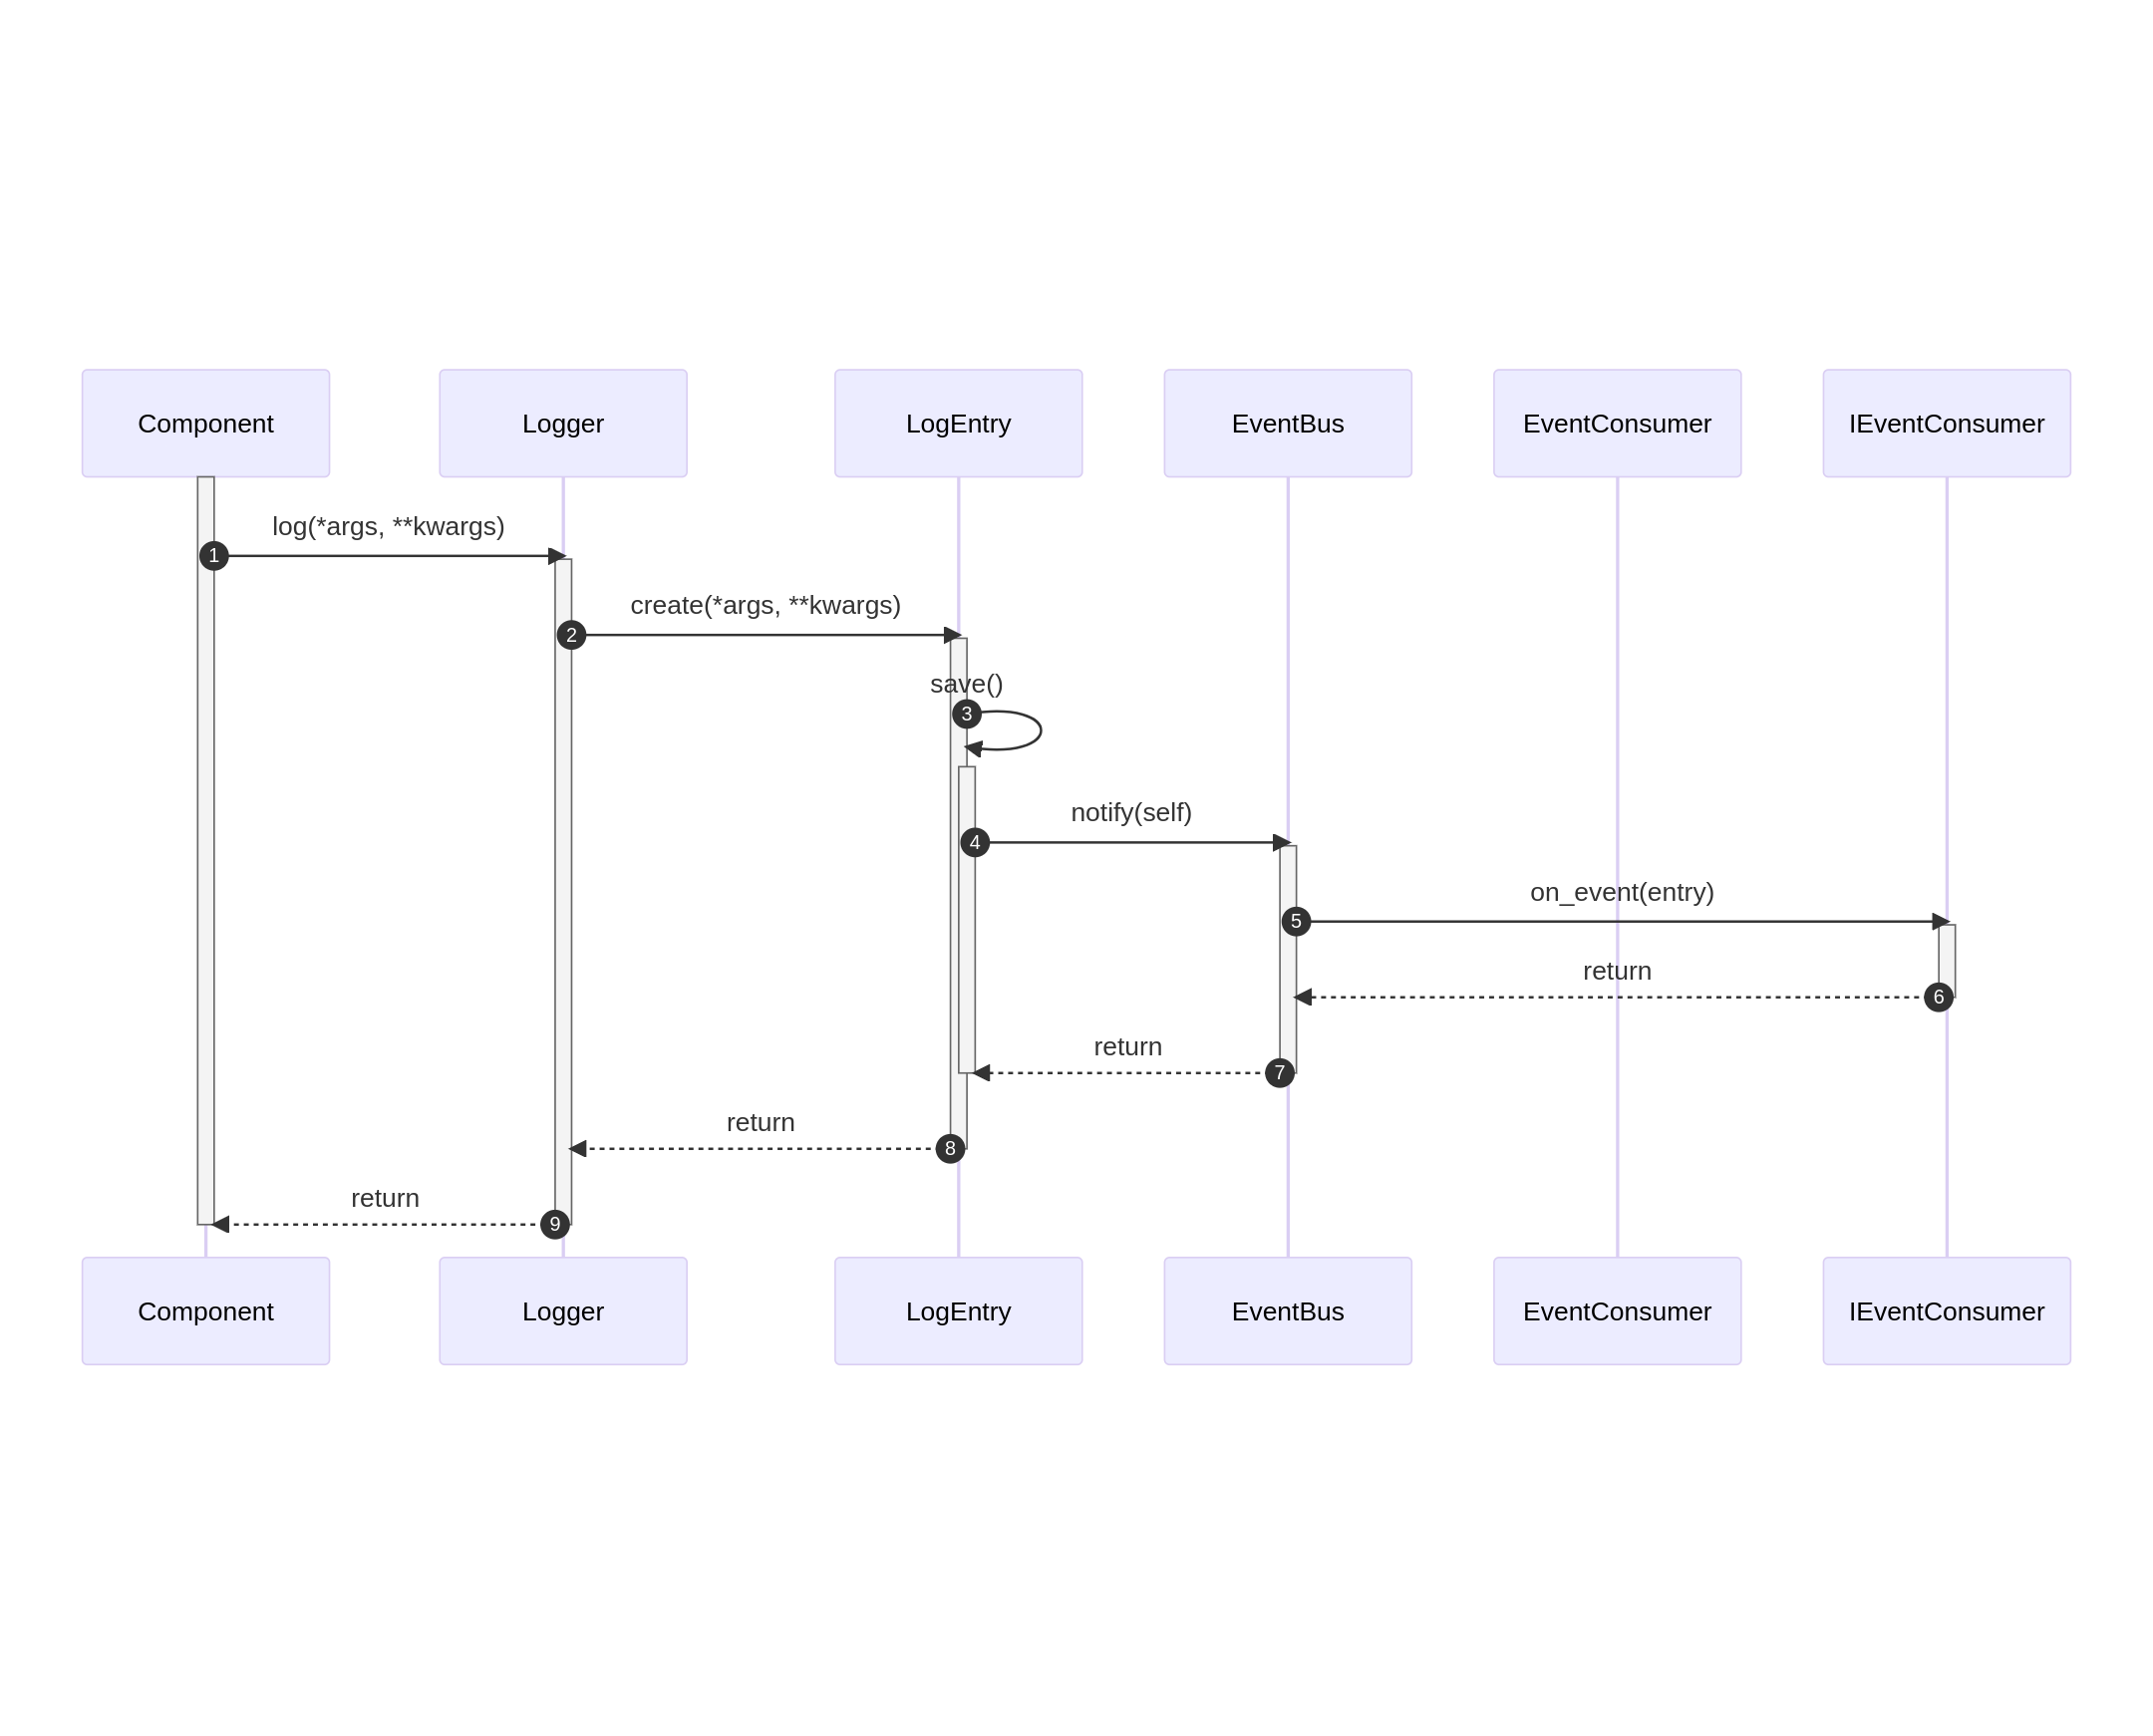
\includegraphics[width=0.75\linewidth]{images/diagrams/eventbus-v1-seq.png}
	\caption{Sequenzdiagramm Variante 1 Eventbus}
	\label{fig:eventbus-v1-seq}
\end{figure}

\subsubsection*{Variante 2}

\begin{figure}[!hb]
	\centering
	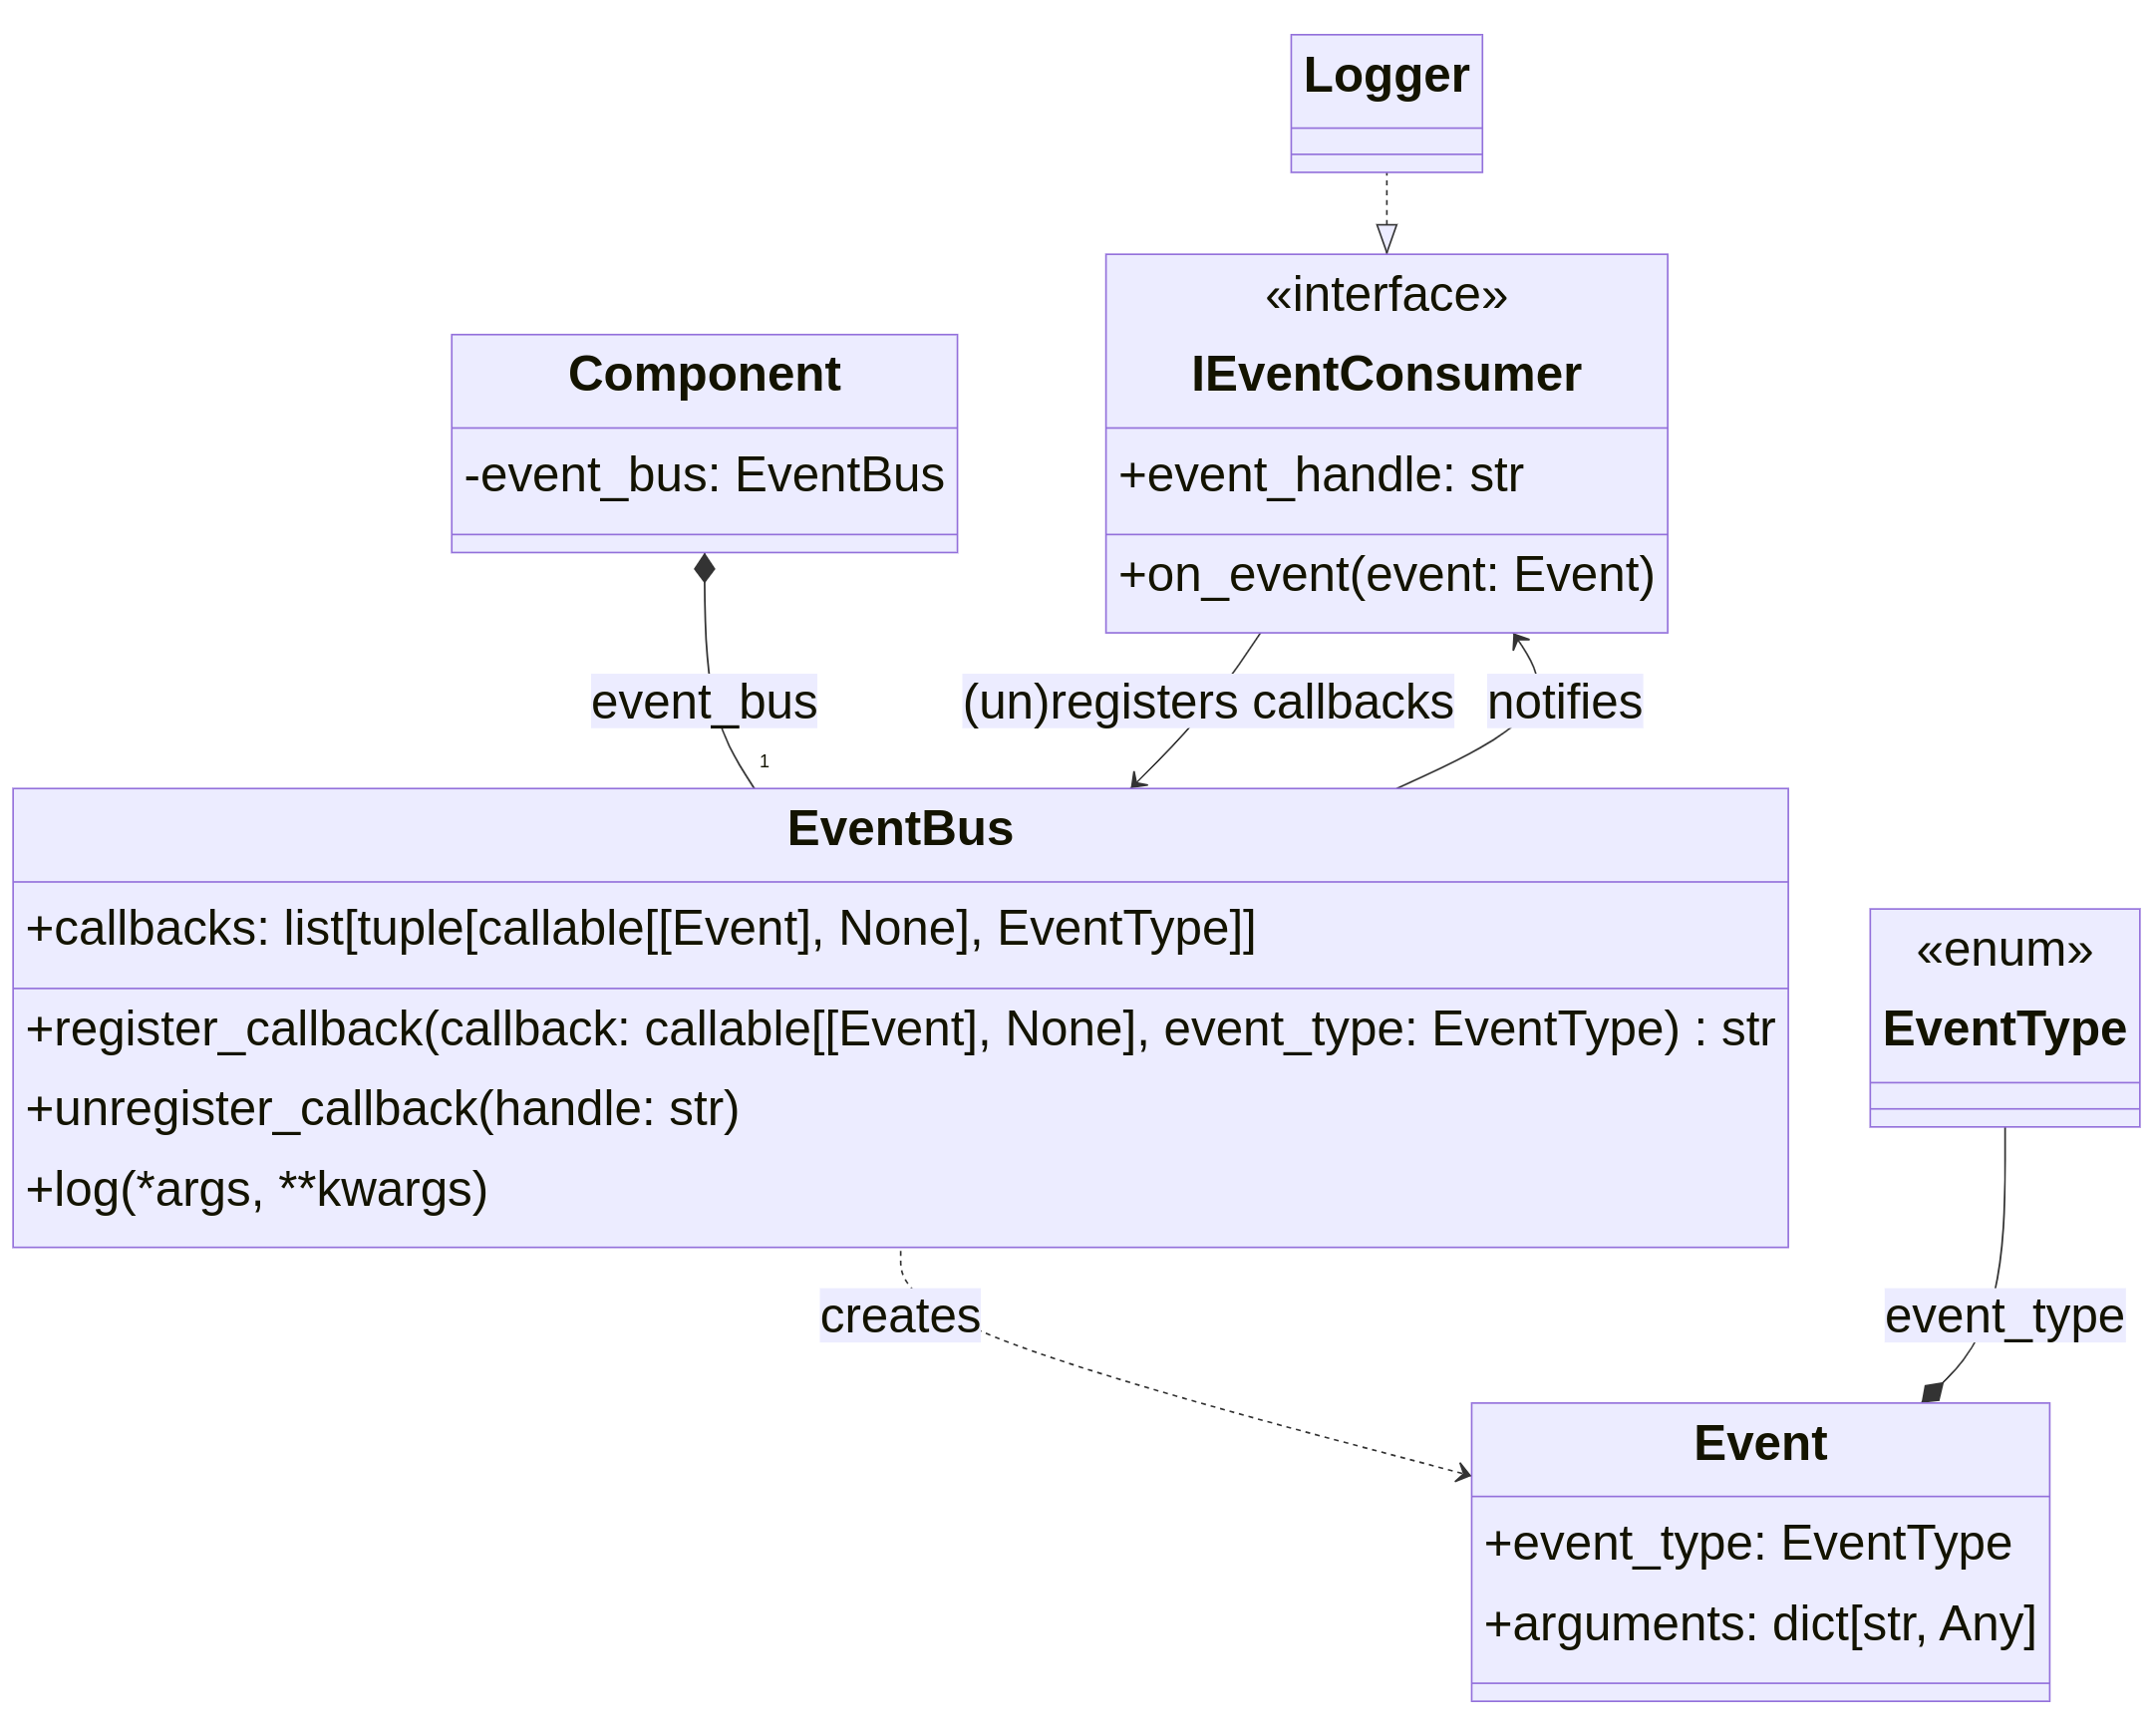
\includegraphics[width=0.75\linewidth]{images/diagrams/eventbus-v2-class.png}
	\caption{Klassendiagramm Variante 2 Eventbus}
	\label{fig:eventbus-v2-class}
\end{figure}

\begin{figure}[!hb]
	\centering
	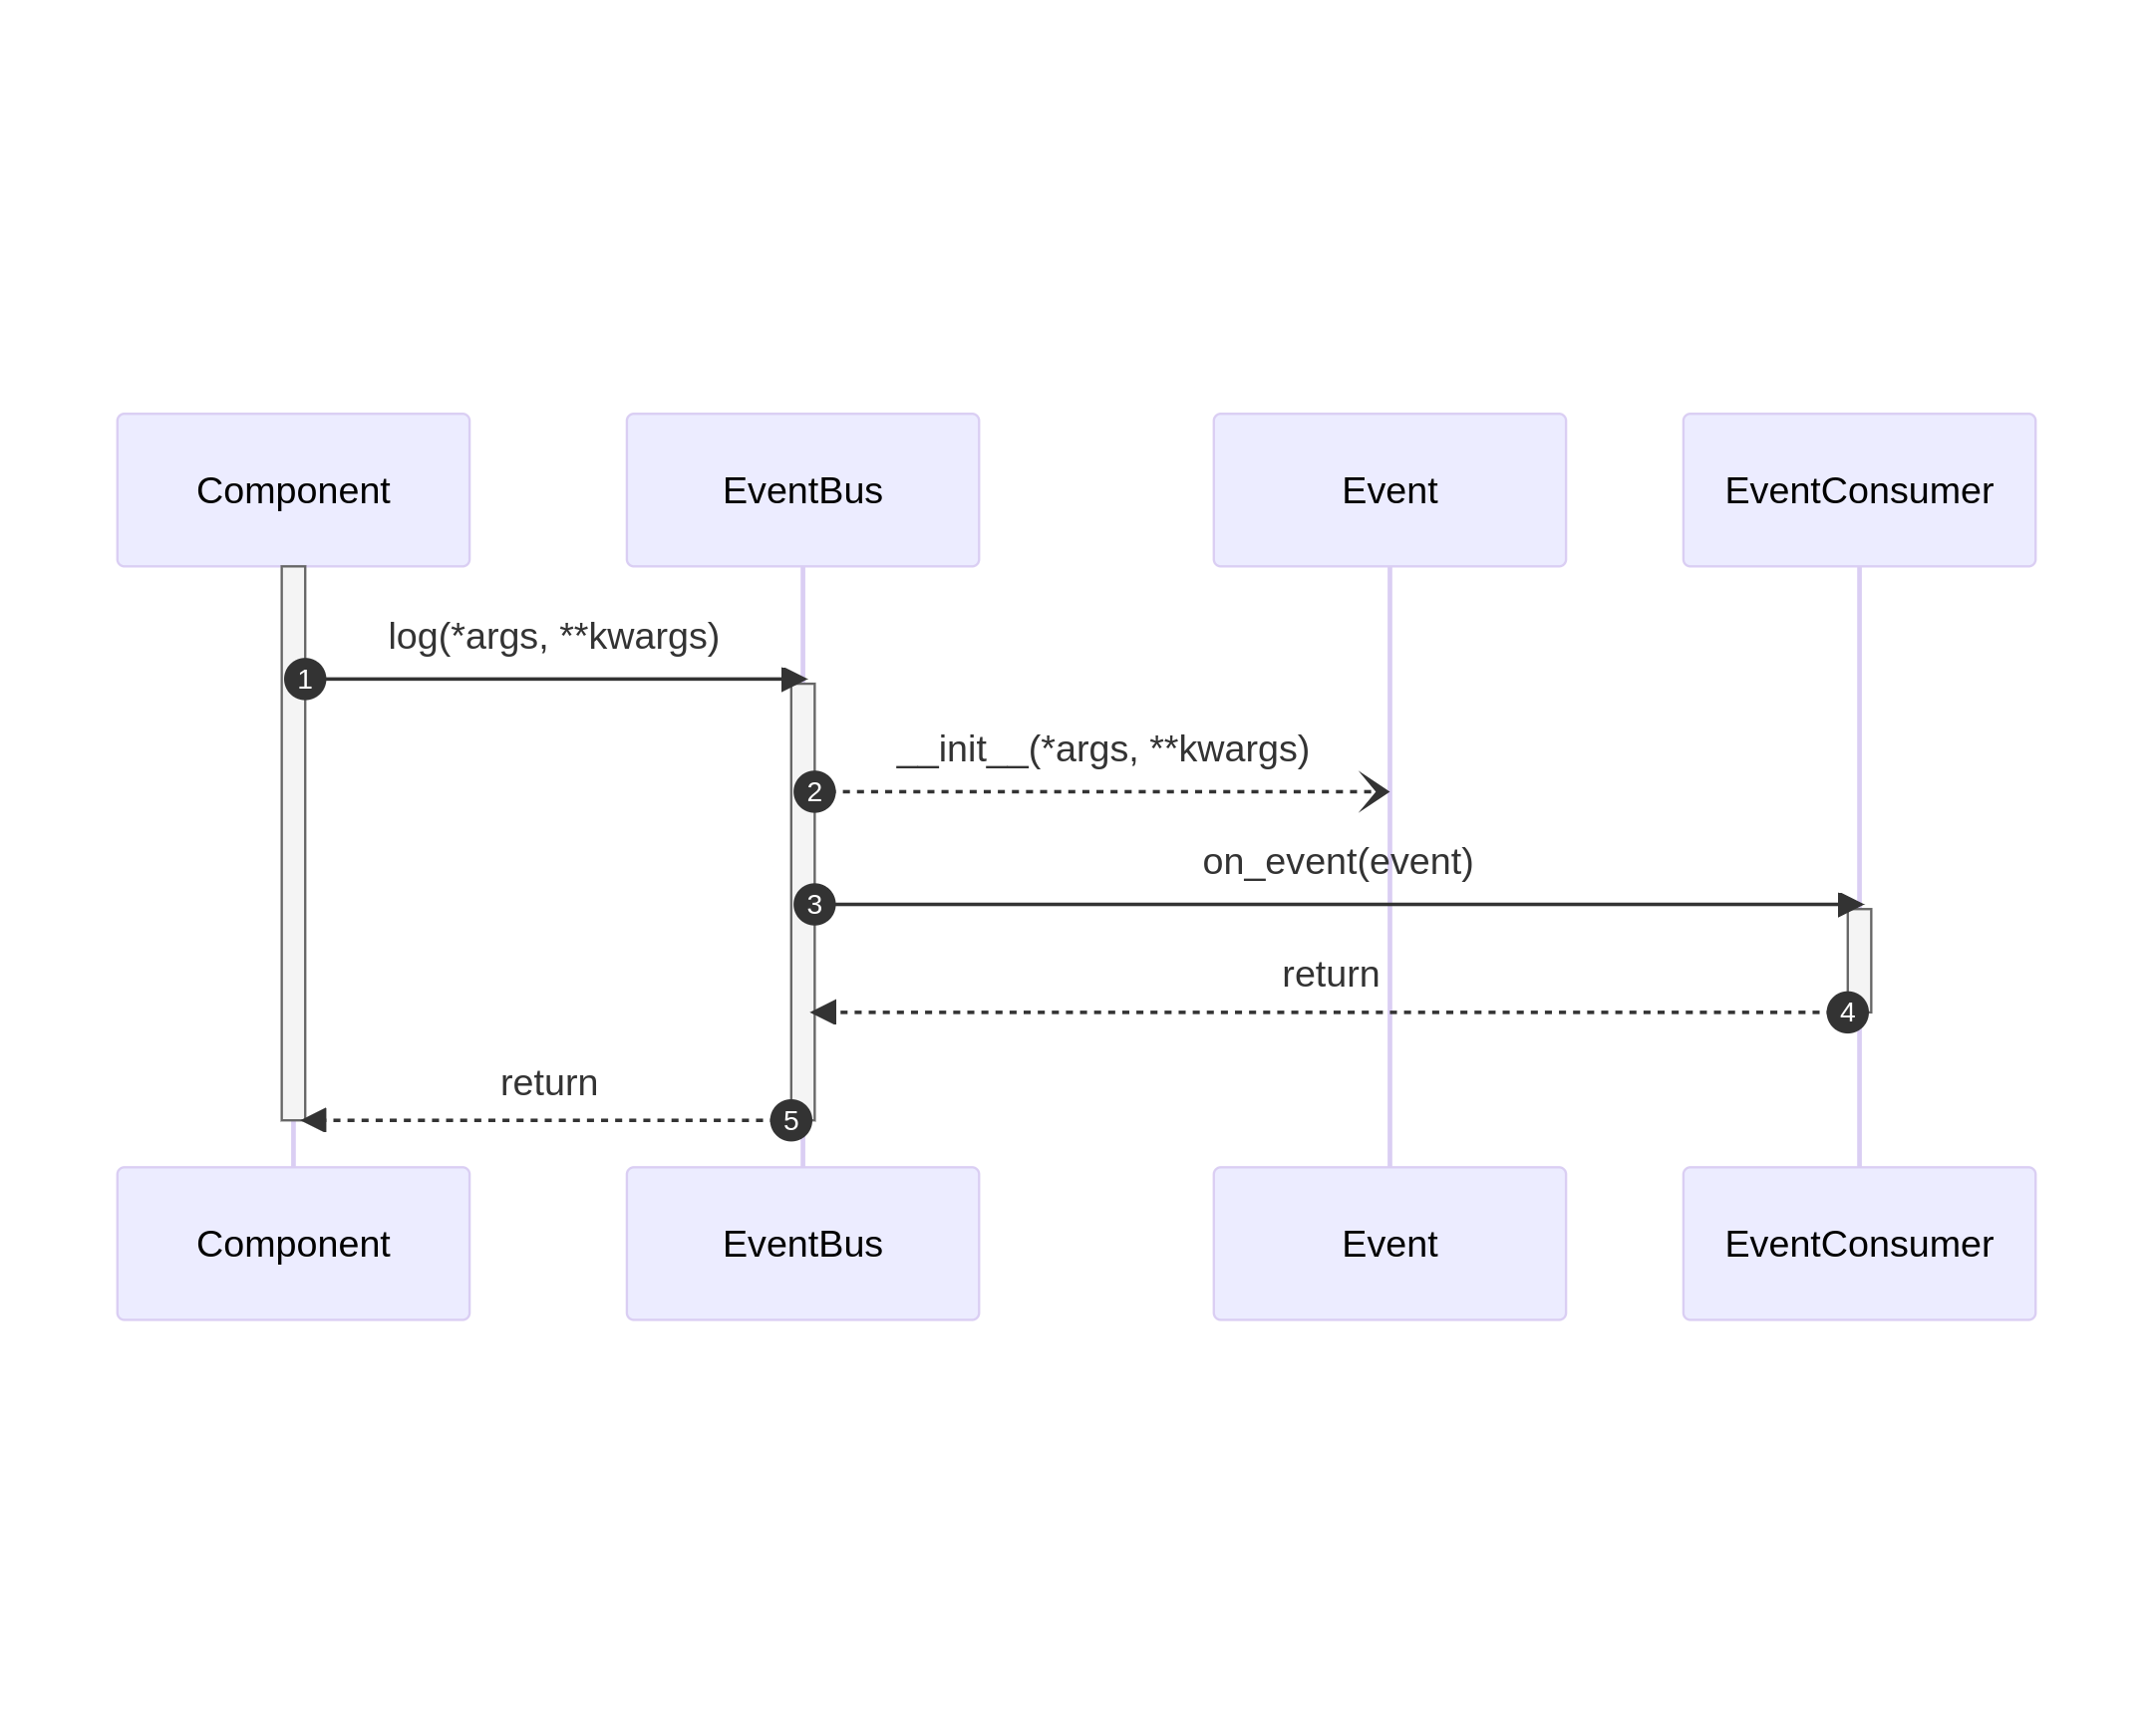
\includegraphics[width=0.75\linewidth]{images/diagrams/eventbus-v2-seq.png}
	\caption{Sequenzdiagramm Variante 2 Eventbus}
	\label{fig:eventbus-v2-seq}
\end{figure}
